\textbf{P3)} \textcolor{red}{[Prueba 1 - 2024-10]} Considere un carrete que rueda sobre un plano rugoso inclinado en ángulo $\phi$. El carrete tiene masa $M$, radio $R_1$ e inercia $I_1$ respecto a su centro. El hilo sale paralelo al plano, pasa sin deslizar por una polea de radio $R_2$ e inercia $I_2$, y sostiene una masa colgante $m$. Asuma que $m$ baja y que el carrete se mueve hacia la derecha.

\begin{enumerate}[a)]
\item Deduzca relaciones entre la aceleración del centro del carrete $a_1$, las aceleraciones angulares del carrete $\alpha_1$ y de la polea $\alpha_2$, y la aceleración con que el cilindro baja $a_m$.
\item Dibuje DCL para cada uno de los tres cuerpos.
\item Escriba las ecuaciones de fuerzas y torques relevantes.
\item Calcule las tensiones en los dos tramos del hilo y la aceleración $a_m$.
\end{enumerate}

\begin{center}
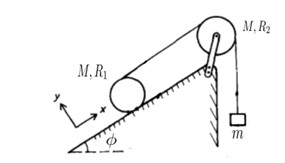
\includegraphics[width=0.55\textwidth]{imagenes/ayudantia_4_ejercicio_3.jpg}
\end{center}

\vspace{0.2cm}
\textbf{Pauta}

Convenciones: sobre el plano, positivo hacia la derecha; para la masa colgante, positivo hacia abajo.

\begin{enumerate}[a)]
\item

Condiciones de no deslizamiento (o de rodadura). Como el carrete rueda sin deslizar y el punto de contacto $C$ tiene velocidad cero (es el CIR del carrete):
\[
v_1=R_1\omega_1.
\]
Por otra parte, el cordel toca al carrete en un punto $P$ que junto al centro $O$ y el punto de contacto $C$ forman un diametro de longitud $2R_1$:
\[
v_m=2R_1\omega_1,
\]
que tambien corresponde a la velocidad con la cual baja la masa colgante $m$.

La polea tambien gira en torno a su centro, de forma que el cordel toca el perimetro sin deslizar:
\[
v_m=R_2\omega_2.
\]
(Para hacer estas deducciones pudimos tambien usar formulas como $\vec{v}_1=\vec{v}_C+\vec{\omega}\times\vec{r}_1$.)

Estas 3 relaciones entre 4 rapideces se pueden escribir como 3 relaciones entre aceleraciones:
\[
a_1=R_1\alpha_1,
\qquad
a_m=2R_1\alpha_1,
\qquad
a_m=R_2\alpha_2.
\]

\item

DCL del carrete:
\begin{itemize}
\item $T_1$ hacia derecha-arriba en $P$,
\item $Mg$ hacia abajo aplicado en $O$,
\item $N$ hacia arriba-izquierda aplicado en $C$,
\item $f$ hacia izquierda-abajo aplicada en $C$.
\end{itemize}
En el diagrama, estas fuerzas deben aparecer con sus lineas de accion claramente trazadas.
DC del carrete: $a_1$ hacia derecha-arriba, $\alpha_1$ en sentido anti-horario.

DCL de la polea:
\begin{itemize}
\item $T_1$ hacia izquierda-abajo en $P'$,
\item $T_2$ hacia abajo aplicado en $P''$,
\item $Mg$ hacia abajo aplicado en $O'$,
\item $F_x,F_y$ aplicadas en $O'$.
\end{itemize}
En el diagrama, estas fuerzas deben aparecer con sus lineas de accion claramente trazadas.
DC de la polea: $\alpha_2$ en sentido anti-horario.

DCL de la masa colgante:
\begin{itemize}
\item $T_2$ hacia arriba,
\item $mg$ hacia abajo.
\end{itemize}
DC de la masa colgante: $a_m$ hacia abajo.

\item \textbf{Ecuaciones}

No se escribiran las ecuaciones de fuerzas de la polea, y la de torques de la masa colgante, porque no son relevantes. Usando ejes inclinados para el carrete:
\[
-Mg\sin\phi-f+T_1=Ma_1,
\]
\[
N-Mg\cos\phi=0,
\]
\[
R_1T_1+R_1f=I_1\alpha_1,
\]
\[
R_2T_2-R_2T_1=I_2\alpha_2,
\]
\[
mg-T_2=ma_m.
\]

(5 ecuaciones para las 8 incognitas $a_1,a_m,\alpha_1,\alpha_2,T_1,T_2,N,f$. Debemos tambien incluir las 3 ecuaciones que resultan de imponer condiciones de no deslizamiento.)


\item \textbf{Resultados}
Descartando la segunda ecuacion y usando las condiciones de no deslizamiento entre las aceleraciones:
\[
-Mg\sin\phi-f+T_1=\left(\frac{M}{2}\right)a_m,
\]
\[
R_1T_1+R_1f=\left(\frac{I_1}{2R_1}\right)a_m,
\]
\[
R_2T_2-R_2T_1=\left(\frac{I_2}{R_2}\right)a_m,
\]
\[
mg-T_2=ma_m.
\]
(4 ecuaciones para las 4 incognitas $a_m,T_1,T_2,f$.)

Combinando las dos primeras ecuaciones para eliminar $f$, y las dos ultimas para eliminar $T_2$:
\[
2R_1T_1-R_1Mg\sin\phi=\left(\frac{R_1M}{2}+\frac{I_1}{2R_1}\right)a_m,
\]
\[
R_2mg-R_2T_1=\left(\frac{I_2}{R_2}+R_2m\right)a_m.
\]

Combinando para eliminar $T_1$:
\[
2R_1R_2mg-R_1R_2Mg\sin\phi=
\left(\frac{R_1R_2M}{2}+\frac{I_1R_2}{2R_1}+\frac{2I_2R_1}{R_2}+2R_1R_2m\right)a_m.
\]

Despejando:
\[
a_m=
\frac{2R_1R_2m-R_1R_2M\sin\phi}{\frac{R_1R_2M}{2}+\frac{I_1R_2}{2R_1}+\frac{2I_2R_1}{R_2}+2R_1R_2m}\,g.
\]

Las tensiones $T_1$ y $T_2$ se pueden despejar ahora facilmente.
\end{enumerate}
